% Path: docs/report_academic_it.tex
\documentclass[12pt,a4paper]{article}

\usepackage[utf8]{inputenc}
\usepackage[T1]{fontenc}
\usepackage[italian]{babel}
\usepackage{geometry}
\usepackage{booktabs}
\usepackage{graphicx}
\usepackage{float}
\usepackage{hyperref}
\usepackage{enumitem}
\usepackage{setspace}
\usepackage{amsmath}
\usepackage{amssymb}
\usepackage{multirow}
\usepackage{array}
\usepackage{caption}
\usepackage{longtable}

\geometry{margin=1in}
\onehalfspacing
\hypersetup{colorlinks=true,linkcolor=black,urlcolor=blue,citecolor=black}

\title{\textbf{Image\_Captioning\_CNN\_LSTM}\\
\large Progetto per il corso di Deep Learning e Modelli Generativi}
\author{Giuseppe Dimonte \\ Matricola 367431}
\date{Anno Accademico 2025/26}

\begin{document}

\begin{titlepage}
\centering
{\Large Università degli Studi di Parma \par}
\vspace{0.2cm}
{\large Dipartimento di Ingegneria e Architettura \par}
\vspace{0.2cm}
{\large Corso di Laurea in Ingegneria Informatica \par}
{\large Curriculum: Intelligenza Artificiale \par}
\vspace{1.2cm}
{\Large \textbf{Deep Learning e Modelli Generativi} \par}
\vspace{0.3cm}
{\large Docente: Prof. Andrea Prati \par}
\vspace{1.2cm}
{\huge \textbf{Image\_Captioning\_CNN\_LSTM} \par}
\vspace{1.2cm}
{\large \textbf{Studente:} Giuseppe Dimonte \par}
{\large \textbf{Matricola:} 367431 \par}
{\large \textbf{Email:} giuseppe.dimonte@studenti.unipr.it \par}
\vfill
{\large Anno Accademico 2025/26 \par}
\end{titlepage}

\tableofcontents
\newpage

\begin{abstract}
Questo elaborato presenta lo sviluppo e la valutazione di un sistema di image captioning basato su architettura CNN-LSTM addestrato sul dataset Flickr8k. Il progetto è stato realizzato come risposta all'assegnamento del corso di Deep Learning e Modelli Generativi e copre l'intera pipeline richiesta: pulizia delle caption, costruzione del vocabolario, preparazione dei file di train/validation/test, definizione dell'architettura, addestramento supervisionato, valutazione quantitativa con metriche BLEU e analisi qualitativa delle caption generate. La parte sperimentale è stata organizzata come confronto controllato tra una configurazione baseline e tre varianti: rimozione dello scheduled sampling, rimozione del label smoothing e fine-tuning della CNN. I risultati mostrano che scheduled sampling e label smoothing migliorano le prestazioni rispetto alle rispettive ablation, mentre il fine-tuning dell'encoder produce il miglior comportamento complessivo, con BLEU-4 pari a 0.0649 contro lo 0.0472 della baseline. Il report discute inoltre i vincoli computazionali imposti da un setup CPU-only, la struttura della repository, i problemi implementativi corretti durante il lavoro e i limiti del sistema finale.
\end{abstract}

\section{Introduzione}

L'image captioning è un problema di apprendimento multimodale in cui un sistema deve produrre una descrizione linguistica di un'immagine. Si tratta di un task non banale perché richiede di integrare due competenze differenti: da un lato l'estrazione di informazione visiva rilevante, dall'altro la generazione di una sequenza testuale coerente e grammaticalmente plausibile. In termini operativi, il problema può essere visto come una mappatura da spazio delle immagini a spazio delle sequenze di token.

Dal punto di vista applicativo, l'image captioning è rilevante in scenari diversi: supporto all'accessibilità, indicizzazione semantica di immagini, interfacce multimodali e sistemi di retrieval avanzato. Dal punto di vista scientifico, il problema è interessante perché costringe a integrare metodi di computer vision e language modeling in un'unica pipeline.

L'obiettivo di questo progetto è implementare un sistema di image captioning basato su CNN-LSTM, in linea con i vincoli dell'assegnamento del corso. Oltre all'implementazione del modello, il lavoro ha richiesto:
\begin{itemize}[leftmargin=*]
    \item la costruzione di una pipeline dati corretta e riproducibile;
    \item la gestione di esperimenti controllati e confrontabili;
    \item la raccolta sistematica di artefatti sperimentali;
    \item la produzione di un report tecnico difendibile su risultati reali e non ipotetici.
\end{itemize}

\section{Traccia dell'assegnamento e obiettivi}

La traccia richiedeva esplicitamente:
\begin{itemize}[leftmargin=*]
    \item l'utilizzo del dataset Flickr8k;
    \item l'implementazione di un'architettura CNN-LSTM;
    \item la pulizia del testo delle caption;
    \item la costruzione e il salvataggio di un dizionario/vocabolario;
    \item l'uso di sequenze tokenizzate compatibili con il decoder LSTM;
    \item la generazione di caption in fase di test mediante decoder linguistico.
\end{itemize}

Di conseguenza, gli obiettivi operativi del progetto sono stati:
\begin{enumerate}[leftmargin=*]
    \item costruire una pipeline dati che trasformi Flickr8k in input riproducibili per il training;
    \item implementare una CNN pre-addestrata per l'estrazione di feature visuali;
    \item implementare un decoder LSTM autoregressivo per la generazione delle caption;
    \item valutare il sistema con metriche standard di image captioning;
    \item misurare l'effetto di alcune scelte di training tramite ablation study.
\end{enumerate}

\section{Formulazione del problema}

Dato un input visivo \(I\), il sistema deve generare una sequenza di parole \(w_1, w_2, \dots, w_T\) che descriva l'immagine. Formalmente, il problema consiste nello stimare:

\[
P(w_1, w_2, \dots, w_T \mid I)
\]

Utilizzando la decomposizione autoregressiva:

\[
P(w_1, w_2, \dots, w_T \mid I) = \prod_{t=1}^{T} P(w_t \mid w_{<t}, I)
\]

Questa formulazione giustifica l'uso di un'architettura encoder-decoder:
\begin{itemize}[leftmargin=*]
    \item l'\textbf{encoder} trasforma l'immagine in una rappresentazione vettoriale informativa;
    \item il \textbf{decoder} stima la probabilità del token successivo dato il contesto testuale già generato e la rappresentazione dell'immagine.
\end{itemize}

\section{Dataset}

\subsection{Flickr8k}

Il dataset utilizzato è Flickr8k, un benchmark classico per l'image captioning. Ogni immagine è accompagnata da cinque caption di riferimento. Questa caratteristica è importante perché consente di valutare una caption generata non rispetto a un'unica descrizione “vera”, ma rispetto a un insieme di descrizioni semanticamente valide.

\subsection{Split e artefatti generati}

Per rendere il workflow riproducibile, il dataset è stato trasformato nei seguenti artefatti:
\begin{itemize}[leftmargin=*]
    \item \texttt{data/vocab.json}
    \item \texttt{data/Flickr8k\_text/train.csv}
    \item \texttt{data/Flickr8k\_text/val.csv}
    \item \texttt{data/Flickr8k\_text/test\_captions.json}
\end{itemize}

Dimensioni osservate:
\begin{itemize}[leftmargin=*]
    \item righe di training: 30000
    \item righe di validation: 5000
    \item immagini di test: 1000
    \item caption di riferimento per immagine in test: 5
\end{itemize}

\section{Preprocessing del testo e costruzione del vocabolario}

Le caption originali sono state preprocessate per rispettare i requisiti della traccia e ridurre la rumorosità linguistica. Il preprocessing applica:
\begin{itemize}[leftmargin=*]
    \item conversione in minuscolo;
    \item rimozione della punteggiatura;
    \item rimozione dei numeri;
    \item rimozione delle parole costituite da una sola lettera;
    \item normalizzazione degli spazi.
\end{itemize}

Dal testo pulito è stato costruito un vocabolario con soglia minima di frequenza. Sono stati aggiunti quattro token speciali:
\begin{itemize}[leftmargin=*]
    \item \texttt{<pad>} per il padding;
    \item \texttt{<bos>} per marcare l'inizio sequenza;
    \item \texttt{<eos>} per marcare la fine sequenza;
    \item \texttt{<unk>} per parole fuori vocabolario.
\end{itemize}

Il vocabolario finale contiene 2985 token.

\subsection{Osservazione metodologica}

Questa fase si è rivelata più critica del previsto. Durante la revisione del progetto è emerso che il parser iniziale delle caption non era coerente con il formato reale di Flickr8k. La correzione di questo punto è stata essenziale per garantire che vocabolario, split ed evaluation fossero costruiti su dati realmente corretti.

\section{Architettura del modello}

\subsection{Encoder CNN}

L'encoder è basato su InceptionV3 pre-addestrata su ImageNet. Il layer finale di classificazione è stato rimosso e sostituito con una proiezione lineare nello spazio di embedding del decoder. In questo modo l'immagine viene trasformata in un vettore compatto che sintetizza il contenuto visivo.

\subsection{Decoder LSTM}

Il decoder è una LSTM a singolo layer. In fase di training riceve in input:
\begin{itemize}[leftmargin=*]
    \item la rappresentazione visiva dell'immagine;
    \item la sequenza di token della caption.
\end{itemize}

Per ogni timestep, un layer lineare finale produce i logits sul vocabolario, consentendo la predizione del token successivo.

\subsection{Perché CNN-LSTM}

L'uso di una CNN per la parte visuale e di una LSTM per la parte linguistica riflette l'impostazione classica dell'image captioning prima della diffusione dei decoder Transformer. In un contesto accademico, questa scelta è particolarmente utile perché il funzionamento dell'encoder-decoder è facilmente interpretabile e pienamente allineato alla traccia del progetto.

\section{Dettagli implementativi}

La repository è organizzata in modo modulare:
\begin{itemize}[leftmargin=*]
    \item \texttt{src/vocab\_builder.py}: parsing delle caption, pulizia del testo, costruzione del vocabolario, esportazione split;
    \item \texttt{src/prepare\_data.py}: script unico per preparazione dei dati;
    \item \texttt{src/dataset.py}: caricamento immagini, conversione caption in token, padding;
    \item \texttt{src/model.py}: definizione di encoder, decoder e wrapper complessivo;
    \item \texttt{src/train.py}: training, validation, checkpointing, resume;
    \item \texttt{src/eval.py}: generazione caption e calcolo BLEU;
    \item \texttt{src/visualize.py}: esportazione di esempi qualitativi;
    \item \texttt{src/ui\_streamlit.py}: demo interattiva opzionale.
\end{itemize}

\subsection{Correzioni strutturali effettuate}

Prima della campagna sperimentale finale sono state effettuate correzioni sostanziali:
\begin{itemize}[leftmargin=*]
    \item correzione del parser delle caption;
    \item generazione automatica dei file mancanti per training e test;
    \item riallineamento della loss alla next-token prediction;
    \item attivazione reale del fine-tuning della CNN;
    \item allineamento dei path tra codice, config e artefatti reali;
    \item introduzione di configurazioni sperimentali separate per confronti controllati.
\end{itemize}

\section{Strategia di training}

Il training implementa le seguenti tecniche:
\begin{itemize}[leftmargin=*]
    \item \textbf{Scheduled sampling}: riduzione graduale del teacher forcing;
    \item \textbf{Label smoothing}: regolarizzazione della distribuzione target;
    \item \textbf{Gradient clipping}: stabilizzazione dell'ottimizzazione;
    \item \textbf{Checkpointing}: salvataggio di \texttt{last.pt} e \texttt{model\_best.pt};
    \item \textbf{Resume}: ripresa del training da checkpoint dopo interruzioni.
\end{itemize}

Questi elementi non sono stati soltanto teorici: nella pratica, la possibilità di riprendere run interrotte si è rivelata indispensabile a causa dei tempi di training su CPU.

\section{Protocollo sperimentale}

\subsection{Ambiente di esecuzione}

Gli esperimenti finali sono stati eseguiti nel seguente ambiente:
\begin{itemize}[leftmargin=*]
    \item ambiente Conda: \texttt{captioning}
    \item eseguibile Python: \texttt{C:\textbackslash Users\textbackslash Giuseppe\textbackslash anaconda3\textbackslash envs\textbackslash captioning\textbackslash python.exe}
    \item versione PyTorch: \texttt{2.9.1+cpu}
    \item dispositivo: CPU
\end{itemize}

\subsection{Esperimenti confrontati}

Sono state confrontate quattro configurazioni:
\begin{enumerate}[leftmargin=*]
    \item \textbf{Baseline}: scheduled sampling e label smoothing attivi;
    \item \textbf{No Scheduled Sampling}: scheduled sampling disattivato;
    \item \textbf{No Label Smoothing}: label smoothing disattivato;
    \item \textbf{Fine-tuning}: fine-tuning della CNN attivato.
\end{enumerate}

Nella comparazione finale tutte le configurazioni sono state eseguite per 5 epoche.

\section{Risultati quantitativi}

\subsection{Metriche BLEU}

\begin{table}[H]
\centering
\caption{Confronto BLEU tra gli esperimenti finali.}
\begin{tabular}{lcccc}
\toprule
Esperimento & BLEU-1 & BLEU-2 & BLEU-3 & BLEU-4 \\
\midrule
Baseline & 0.2553 & 0.1556 & 0.0928 & 0.0472 \\
No Scheduled Sampling & 0.2232 & 0.1242 & 0.0717 & 0.0396 \\
No Label Smoothing & 0.2404 & 0.1435 & 0.0809 & 0.0394 \\
Fine-tuning & 0.3301 & 0.2022 & 0.1189 & 0.0649 \\
\bottomrule
\end{tabular}
\end{table}

\subsection{Riassunto del training}

\begin{table}[H]
\centering
\caption{Riassunto del comportamento in training e validation.}
\begin{tabular}{lccc}
\toprule
Esperimento & Best Val Loss & Final Train Loss & Final Val Loss \\
\midrule
Baseline & 4.1927 & 4.8016 & 4.2332 \\
No Scheduled Sampling & 4.0106 & 3.5373 & 4.0234 \\
No Label Smoothing & 3.5029 & 4.0860 & 3.5738 \\
Fine-tuning & 3.6614 & 4.7512 & 4.2861 \\
\bottomrule
\end{tabular}
\end{table}

\section{Discussione dei risultati}

\subsection{Baseline}

La baseline costituisce il riferimento sperimentale del progetto. Include sia scheduled sampling sia label smoothing e raggiunge BLEU-4 pari a 0.0472.

\subsection{Rimozione dello scheduled sampling}

Rimuovendo lo scheduled sampling si osserva una riduzione di tutte le metriche BLEU. Questo è un risultato rilevante perché, nonostante la training loss risulti inferiore rispetto alla baseline, la qualità finale delle caption peggiora. Il fenomeno suggerisce che il modello apprenda meglio il training set ma generalizzi peggio in generazione autoregressiva.

\subsection{Rimozione del label smoothing}

Anche la rimozione del label smoothing peggiora le metriche rispetto alla baseline. La tecnica sembra quindi contribuire positivamente alla stabilità e alla qualità finale della generazione.

\subsection{Fine-tuning della CNN}

Il fine-tuning dell'encoder produce il miglior comportamento complessivo:
\begin{itemize}[leftmargin=*]
    \item BLEU-1 = 0.3301
    \item BLEU-2 = 0.2022
    \item BLEU-3 = 0.1189
    \item BLEU-4 = 0.0649
\end{itemize}

Questo indica che l'adattamento della CNN al task di image captioning fornisce un vantaggio misurabile.

\section{Analisi qualitativa}

Per la documentazione finale sono stati selezionati tre esempi rappresentativi.

\begin{figure}[H]
    \centering
    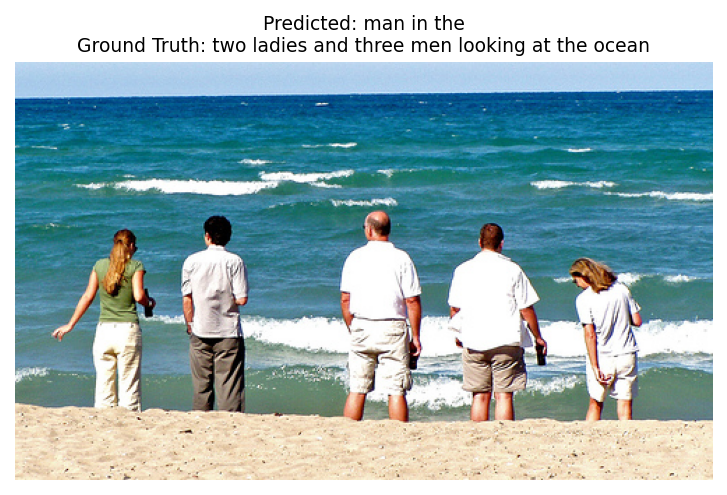
\includegraphics[width=0.8\textwidth]{selected_figures/baseline_example.png}
    \caption{Esempio della baseline. La predizione è collegata alla scena ma rimane generica e non cattura la descrizione completa.}
    \label{fig:baseline_academic}
\end{figure}

\begin{figure}[H]
    \centering
    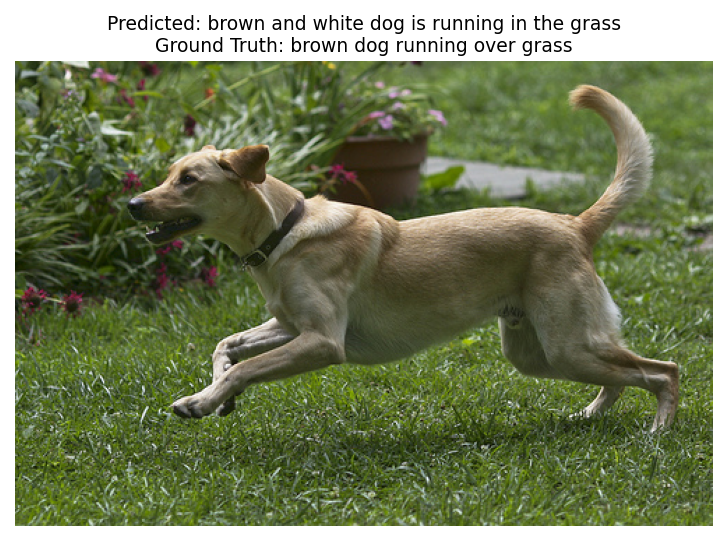
\includegraphics[width=0.8\textwidth]{selected_figures/finetune_example.png}
    \caption{Esempio del modello fine-tuned. La caption generata identifica correttamente l'oggetto principale e l'azione.}
    \label{fig:finetune_academic}
\end{figure}

\begin{figure}[H]
    \centering
    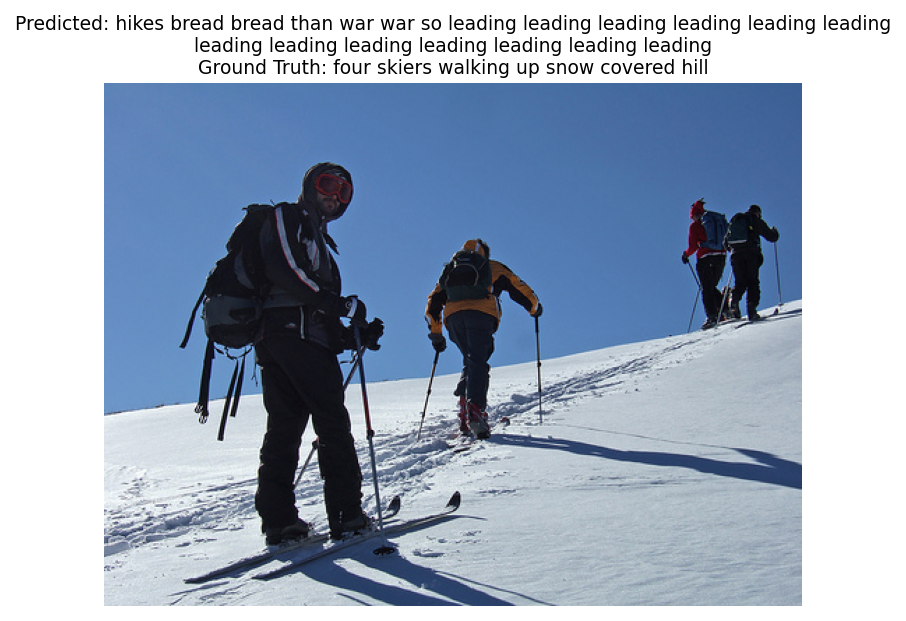
\includegraphics[width=0.8\textwidth]{selected_figures/failure_case.png}
    \caption{Failure case. L'output contiene ripetizioni e deriva semantica, mostrando un limite residuo del sistema.}
    \label{fig:failure_academic}
\end{figure}

\subsection{Interpretazione qualitativa}

Gli esempi qualitativi confermano quanto emerso dalle metriche:
\begin{itemize}[leftmargin=*]
    \item la baseline tende a produrre caption semplici o incomplete;
    \item il modello fine-tuned è più preciso nella descrizione di oggetti e azioni;
    \item rimangono casi in cui il decoder collassa in sequenze ripetitive o semanticamente scorrette.
\end{itemize}

\section{Vincoli computazionali e riproducibilità}

L'intera campagna sperimentale è stata eseguita su CPU. Questo ha avuto implicazioni concrete:
\begin{itemize}[leftmargin=*]
    \item tempi di addestramento elevati;
    \item necessità di gestire i run in più sessioni;
    \item utilizzo reale del resume da checkpoint;
    \item pianificazione rigorosa degli esperimenti per evitare spreco di tempo macchina.
\end{itemize}

Dal punto di vista della riproducibilità, il progetto include:
\begin{itemize}[leftmargin=*]
    \item script di preparazione dati;
    \item config dedicate per ogni esperimento;
    \item log di training ed evaluation;
    \item checkpoint del best model e dell'ultimo stato;
    \item file JSON delle predizioni;
    \item figure qualitative per ogni configurazione.
\end{itemize}

\section{Limiti del progetto}

\begin{itemize}[leftmargin=*]
    \item Flickr8k è un dataset relativamente piccolo per image captioning;
    \item l'architettura CNN-LSTM è un approccio classico ma non più allo stato dell'arte;
    \item la qualità assoluta delle caption resta limitata;
    \item alcuni output risultano ancora generici o instabili.
\end{itemize}

\section{Sviluppi futuri}

Tra i possibili sviluppi futuri:
\begin{itemize}[leftmargin=*]
    \item confronto con decoder Transformer;
    \item utilizzo di beam search;
    \item addestramento su dataset più grandi;
    \item valutazione con metriche aggiuntive oltre a BLEU.
\end{itemize}

\section{Conclusioni}

Il progetto ha implementato una pipeline completa di image captioning con CNN-LSTM su Flickr8k, includendo preprocessing, costruzione del vocabolario, training, validation, evaluation e analisi qualitativa. I risultati mostrano che scheduled sampling e label smoothing migliorano le prestazioni rispetto alle rispettive ablation, mentre il fine-tuning della CNN fornisce il miglior risultato finale. L'insieme di codice, log, checkpoint, figure e file di risultato rende il progetto sufficientemente completo per una consegna accademica strutturata.

\section*{Riferimenti}

\begin{thebibliography}{9}

\bibitem{vinyals2015show}
O. Vinyals, A. Toshev, S. Bengio, D. Erhan,
\textit{Show and Tell: A Neural Image Caption Generator},
CVPR, 2015.

\bibitem{flickr8k}
Flickr8k Dataset,
\url{https://github.com/goodwillyoga/Flickr8k_dataset}

\bibitem{inception}
C. Szegedy et al.,
\textit{Rethinking the Inception Architecture for Computer Vision},
CVPR, 2016.

\end{thebibliography}

\section*{Appendice: artefatti prodotti}

I principali artefatti finali del progetto sono:
\begin{itemize}[leftmargin=*]
    \item \texttt{results/metrics\_summary.csv}
    \item \texttt{results/experiment\_summary.csv}
    \item \texttt{results/*\_predictions.json}
    \item \texttt{logs/*}
    \item \texttt{figures/*}
    \item \texttt{LAB\_LOG.md}
\end{itemize}

\end{document}
